\subsection{Пересчет упрощенной электронной таблицы используя Z3Py}

\renewcommand{\CURPATH}{equations/spreadsheet}

% TODO cite?
Есть неплохая задача\footnote{\url{http://thesz.livejournal.com/280784.html}}:
напишите программу для пересчета упрощенной электронной таблицы, вот как такой:

\lstinputlisting{\CURPATH/test1}

Результат должен быть такой:

\lstinputlisting{\CURPATH/test1_result}

Как выясняется, хотя это и слишком, но это может решить MK85 без всякого труда:

\lstinputlisting{\CURPATH/spreadsheet_MK85.py}

( \url{.../spreadsheet_MK85.py} )

Всё что мы делаем это создаем пачку переменных для каждой ячейки, с названиями 
A0, B1, итд, целочисленного типа.
Все они сохраняются в словаре \textit{cells[]}.
Ключ это строка.
Затем мы парсим все строки из ячеек и добавляем их в список констрайнтов, в случае числа в ячейке: \textit{A0=123},
либо, в случае выражения в ячейке: \textit{A0=B1+C2}.
Тут есть небольшая подготовка строк: строка вроде \textit{A0+B2} становится \textit{cells["A0"]+cells["B2"]}.

Затем строка обрабатыватся Питоновским методом \textit{eval()}, который очень опасен
\footnote{\url{http://stackoverflow.com/questions/1832940/is-using-eval-in-python-a-bad-practice}}:
представьте, если конечный пользователь добавить в ячейку строку с каким-нибудь другим выражением?
Тем не менее, это хорошо служит нашим целям, потому что это простейший способ передать строку с выражением в Z3.

\subsubsection{Z3}

Исходный код почти такой же:

\lstinputlisting{\CURPATH/spreadsheet_Z3_1.py}

( \url{...spreadsheet/spreadsheet_Z3_1.py} )

\subsubsection{Unsat core}

Теперь проблема: что если здесь есть циркулярная (круговая) зависимость? Например:

\lstinputlisting{\CURPATH/test_circular}

Первые две ячейки последнего ряда (C0 и C1) завязаны друг на друга.
Наша программа просто скажет ``unsat'', означая, что она не смогла удовлетворить все констрайнты.
Мы не можем это использовать как сообщение об ошибке для конечного пользователя, потому что от него мало толка.

Хотя, мы можем вытащить \textit{unsat core}, т.е., список переменных, которые для Z3 являются конфликтующими.

\begin{lstlisting}
...
s=Solver()
s.set(unsat_core=True)
...
        # add constraint:
        s.assert_and_track(e, coord_to_name(cur_R, cur_C))
...
if result=="sat":
...
else:
    print s.unsat_core()
\end{lstlisting}

( \url{.../spreadsheet_Z3_2.py} )

Нам нужно явно включить поддержку unsat core и использовать \textit{assert\_and\_track()} вместо метода \textit{add()},
потому что эта возможность замедляет весь процесс, и по умолчанию отключена.
Это работает:

\begin{lstlisting}
 % python 2.py test_circular
unsat
[C0, C1]
\end{lstlisting}

Вероятно, эти переменные могут быть удалены из двухмерного массива, маркированы как \textit{unresolved},
и вся таблица могла бы быть пересчитанной заново.

\subsubsection{Нагрузочное тестирование}

Как сгенерировать большую случайную электронную таблицу?
Вот что мы можем сделать.
В начале создаем случайный \ac{DAG}, как вот этот:

\begin{figure}[H]
\centering
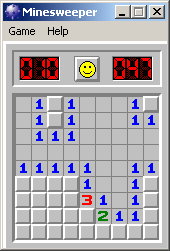
\includegraphics[width=\textwidth]{\CURPATH/1.png}
\caption{Случайный DAG}
\end{figure}

Стрелки определяют потоки информации.
Так что узел графа, который не имеет входящих стрелок (indegree=0), может быть установлен в случайное число.
Затем мы используем топологическую сортировку для поиска зависимостей между узлами графа.
Затем мы назначаем имена ячеек каждому узлу.
Затем мы генерируем случайное выражение со случайными операциями/числами/ячейками, используя информацию
полученную из топологически отсортированного графа.

\begin{lstlisting}[label=Wolfram Mathematica]
(* Utility functions *)
In[1]:= findSublistBeforeElementByValue[lst_,element_]:=lst[[ 1;;Position[lst, element][[1]][[1]]-1]]

(* Input in 1..∞ range. 1->A0, 2->A1, etc *)
In[2]:= vertexToName[x_,width_]:=StringJoin[FromCharacterCode[ToCharacterCode["A"][[1]]+Floor[(x-1)/width]],ToString[Mod[(x-1),width]]]

In[3]:= randomNumberAsString[]:=ToString[RandomInteger[{1,1000}]]

In[4]:= interleaveListWithRandomNumbersAsStrings[lst_]:=Riffle[lst,Table[randomNumberAsString[],Length[lst]-1]]

(* We omit division operation because micro-spreadsheet evaluator can't handle division by zero *)
In[5]:= interleaveListWithRandomOperationsAsStrings[lst_]:=Riffle[lst,Table[RandomChoice[{"+","-","*"}],Length[lst]-1]]

In[6]:= randomNonNumberExpression[g_,vertex_]:=StringJoin[interleaveListWithRandomOperationsAsStrings[interleaveListWithRandomNumbersAsStrings[Map[vertexToName[#,WIDTH]&,pickRandomNonDependentVertices[g,vertex]]]]]

In[7]:= pickRandomNonDependentVertices[g_,vertex_]:=DeleteDuplicates[RandomChoice[findSublistBeforeElementByValue[TopologicalSort[g],vertex],RandomInteger[{1,5}]]]

In[8]:= assignNumberOrExpr[g_,vertex_]:=If[VertexInDegree[g,vertex]==0,randomNumberAsString[],randomNonNumberExpression[g,vertex]]

(* Main part *) 
(* Create random graph *)
In[21]:= WIDTH=7;HEIGHT=8;TOTAL=WIDTH*HEIGHT
Out[21]= 56

In[24]:= g=DirectedGraph[RandomGraph[BernoulliGraphDistribution[TOTAL,0.05]],"Acyclic"];

...

(* Generate random expressions and numbers *)
In[26]:= expressions=Map[assignNumberOrExpr[g,#]&,VertexList[g]];

(* Make 2D table of it *)
In[27]:= t=Partition[expressions,WIDTH];

(* Export as tab-separated values *)
In[28]:= Export["/home/dennis/1.txt",t,"TSV"]
Out[28]= /home/dennis/1.txt

In[29]:= Grid[t,Frame->All,Alignment->Left]
\end{lstlisting}


Вот вывод ф-ции \textit{Grid[]}:

\begin{center}
\begin{tabular}{ | l | l | l | l | l | l | l |}
\hline
846 & 499 & A3*913-H4 & ... & ... & ... & ... \\
\hline
B4*860+D2 & 999 & 59 & ... & ... & ... & ... \\
\hline
G6*379-C3-436-C4-289+H6 & 972 & 804 & ... & ... & ... & ... \\
\hline
F2 & E0 & B6-731-D3+791+B4*92+C1 & ... & ... & ... & ... \\
\hline
519 & G1*402+D1*107*G3-458*A1 & D3 & ... & ... & ... & ... \\
\hline
F5-531+B5-222*E4 & 9 & B5+106*B6+600-B1 & ... & ... & ... & ... \\
\hline
C3-956*A5 & G4*408-D3*290*B6-899*G5+400+F1 & B2-701+H6 & ... & ... & ... & .. \\
\hline
B4-792*H4*407+F6-425-E1 & D2 & D3 & ... & ... & ... & ... \\
\hline
\end{tabular}
\end{center}



Используя этот скрипт, я могу сгенерировать случайную электронную таблицу из $26 \cdot 500=13000$ ячеек,
которая затем обрабатывается Z3 несколько секунд.

\subsubsection{Файлы}

Файлы, включая файл для Mathematica: \url{.../spreadsheet}.

